\section{Auswertung}
\label{sec:auswertung}
In diesem Kapitel werden die aufgenommenen Messwerte ausgewertet.
\subsection{Zählrohr Charakterristik}
\label{sec:characteristik}
In diesem Abschnitt wird die sogenannte Charakeristik des Geiger-Müller-Zählrohres ermittelt. Dazu wird der
Abstand der Strahlungsquelle so gewählt, das die Impulsrate bei etwa $\SI{10000}{Imp/min}$ liegt um eine zu große 
Ungenauigkeit durch Totzeiten zu vermeiden. Da die Messwerte poissonverteilt sind wird der Fehler über \autoref{eq:poisson}
\begin{figure}
    \centering
    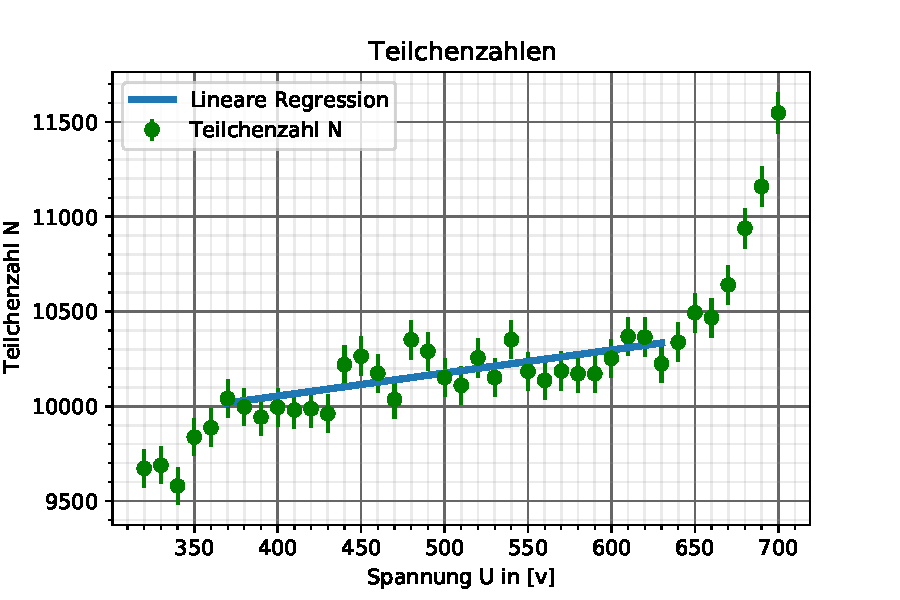
\includegraphics{kennlinie.pdf}
    \caption{Teilchenzahlen im Geiger-Müller-Zählrohr}
    \label{fig:teilchenzahl}
  \end{figure}
Um die Plateau-Steigung zu ermittlen wurde mittels linearer Regression ein Polynom ersten Grades durch die 
Messpunkte gelegt:
\begin{center}
  $f(x)=ax+b$ $\rightarrow$ $D_f=\{x\in\mathbb{R} \vert 360\le x\le620\}$    
\end{center}
mit folgenden Parametern:
\begin{center}
  $a=1.215\pm0.256 \frac{1}{V} $\\
  $b=9567.924\pm125.414 $
\end{center}
Das Plateau hat eine Länge von etwa $\SI{260}{V}$ im Bereich von $\SI{360}{V}$ bis $\SI{620}{V}$ die Steigung 
ergibt sich aus:
\begin{center}
 $\frac{f(x_2)-f(x_1)}{x_2-x_1}=\frac{((1.014\pm0.017)\times 10^4-1.002\pm0.016)\times 10^4}{470 V-370 V}=\SI{1,215\pm0,256}{\frac{\%}{100}}$.
\end{center}
Die verwendeten Messwerte sind:
\begin{table}
    
  \centering
  \caption{Gemessene Impulse pro Zeitintervall in Abhängingkeit von der Spannung}
  \sisetup{table-format=1.2}
  \begin{tabular}{S[table-format=3.2] S S S S [table-format=3.2]}
   % \label{tab:werteTeilchenzahlen}
    \toprule
    {$U$[V]} & {$N$[Imp/min]}\\
    \midrule
    320  &  {$$9672  \pm  98$$}\\
    330  &  {$$9689  \pm  98$$}\\
    340  &  {$$9580  \pm  98$$}\\
    350  &  {$$9837  \pm  99$$}\\
    360  &  {$$9886  \pm  99$$}\\
    370  &  {$$10041 \pm 100$$}\\
    380  &  {$$9996  \pm 100$$}\\
    390  &  {$$9943  \pm 100$$}\\
    400  &  {$$9995  \pm 100$$}\\
    410  &  {$$9980  \pm 100$$}\\
    420  &  {$$9986  \pm 100$$}\\
    430  &  {$$9960  \pm 100$$}\\
    440  &  {$$10219 \pm 101$$}\\
    450  &  {$$10264 \pm 101$$}\\
    460  &  {$$10174 \pm 101$$}\\
    470  &  {$$10035 \pm 100$$}\\
    480  &  {$$10350 \pm 102$$}\\
    490  &  {$$10290 \pm 101$$}\\
    500  &  {$$10151 \pm 101$$}\\
    510  &  {$$10110 \pm 101$$}\\
    520  &  {$$10255 \pm 101$$}\\
    530  &  {$$10151 \pm 101$$}\\
    540  &  {$$10351 \pm 102$$}\\
    550  &  {$$10184 \pm 101$$}\\
    560  &  {$$10137 \pm 101$$}\\
    570  &  {$$10186 \pm 101$$}\\
    580  &  {$$10171 \pm 101$$}\\
    590  &  {$$10171 \pm 101$$}\\
    600  &  {$$10253 \pm 101$$}\\
    610  &  {$$10368 \pm 102$$}\\
    620  &  {$$10365 \pm 102$$}\\
    630  &  {$$10224 \pm 101$$}\\
    640  &  {$$10338 \pm 102$$}\\
    650  &  {$$10493 \pm 102$$}\\
   660  &  {$$10467 \pm 102$$}\\
   670  &  {$$10640 \pm 103$$}\\
     680  &  {$$10939 \pm 105$$}\\
    690  &  {$$11159 \pm 106$$}\\
    700  &  {$$11547 \pm 107$$}\\
\bottomrule
  
  \end{tabular}
\end{table}
Der zu jedem Messwert gehörende Fehler berechnet sich über die Poissonverteilung:
\begin{center}
  \begin{equation}
      \label{eq:poisson}
      \Delta N=\sqrt{N}
      \end{equation}
\end{center}
\subsection{Totzeit des Zählrohres}
\label{sec:totzeit}
An dieser Stelle wird zunächst mithilfe eines Oszilloskopes die Totzeit des Geiger-Müller-Zählrohres
abgeschätzt und anschließend mit der Zwei-Quellen-Methode genauer vermessen bzw. abgeschätzt. 
\subsubsection{Totzeitbestimmung mit dem Oszilloskop}
\label{sec:totzeitO}
In \autoref{fig:oszilloskop} ist die Bildröhre eines Oszilloskopes zu sehen. Die Totzeit ist der Raum 
zwischen den ersten beiden Signalen. Da das Oszilloskop auf 100µs/DIV eingestellt ist und die beiden Signale 
etwa eine Unterteilung (DIV) auseinander liegen wird die Totzeit auf $T \approx 100\mu s$ geschätzt.
\begin{figure}
  \centering
  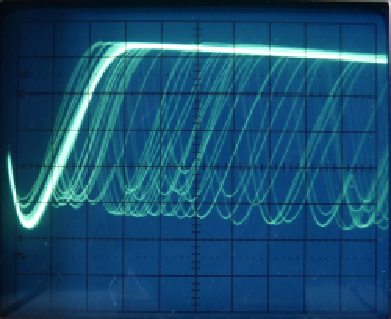
\includegraphics{oszilloskop.pdf}
  \caption{Signal am Geiger-Müller-Zählrohr 100µs/DIV Quelle: 1. TU-Dortmund, V703 Das Geiger-Müller-Zählrohr}
  \label{fig:oszilloskop}
\end{figure}
\subsubsection{Totzeitbestimmung mit der Zwei-Quellen-Methode}
\label{sec:totzeitZ}
Die Totzeit lässt sich mit der Näherungsformel \autoref{eq:totzeit} aus den Messwerten 
\autoref{sec:werteTotzeit} für $N_1$, $N_2$ und $N_{1+2}$ sofort ermittlen, es folgt also mit:
\begin{center}
  $N_1=96041 \frac{Imp}{120 s}$\\
  $N_2=76518 \frac{Imp}{120 s}$\\
  $N_{1+2}=158479 \frac{Imp}{120 s}$
\end{center}
\begin{center}
  $T=(110\pm50) \mu s$
\end{center}
Der entsprechende Fehler wurde mit der Gaußschen-Fehlerfortpflanzung ermittelt.
Dazu wurden folgende Ableitungen verwendet:
\begin{center}
  \begin{equation}
    \label{eq:gaussfehler}  
  \sigma_x=\sqrt{(\frac{\partial f}{\partial x_1})^2\sigma_{x_1}^2+(\frac{\partial f}{\partial x_2})^2\sigma_{x_2}^2+...+(\frac{\partial f}{\partial x_n})^2\sigma_{x_n}^2}
  \end{equation}
  \end{center}
\begin{center}
  $\frac{\partial T}{\partial N_1}=\dfrac{c-b}{2ba^2}$\\
\end{center}
\begin{center}
  $\frac{\partial T}{\partial N_2}=\dfrac{c-a}{2ab^2}$\\
\end{center}
\begin{center}
  $\frac{\partial T}{\partial N_{1+2}}=-\dfrac{1}{2ab}$
\end{center}

\subsection{Ladung pro einfallendem Teilchen}
\label{sec:ladung}
Im folgenden Diagramm \autoref{fig:ladungProTeilchen} ist die Anzahl der Ladungen $Z$ die durch ein einziges einfallendes Teilchen ausgelöst
wurden gegen die Spannung aufgetragen. Die Zahl $Z$ lässt sich mit diesen Werten:
\begin{table}
    
  \centering
  \caption{Messwerte des Stromes}
  \sisetup{table-format=1.2}
  \begin{tabular}{S[table-format=3.2] S S S S  [table-format=3.2]}
  
    \toprule
    {$U$[V]} & {$I$[µA]}\\
    \midrule
    350 &   {$$0.3 \pm 0.05$$}\\
    400	&   {$$0.4 \pm 0.05$$}\\
    450	&   {$$0.7 \pm 0.05$$}\\
    500	&   {$$0.8 \pm 0.05$$}\\
    550	&   {$$1.0 \pm 0.05$$}\\
    600	&   {$$1.3 \pm 0.05$$}\\
    650	&   {$$1.4 \pm 0.05$$}\\
    700	&   {$$1.8 \pm 0.05$$}\\
\bottomrule
  
  \end{tabular}
\end{table}  
direkt über \autoref{eq:zaehlrohrstrom} berechnen
\begin{figure}
  \centering
  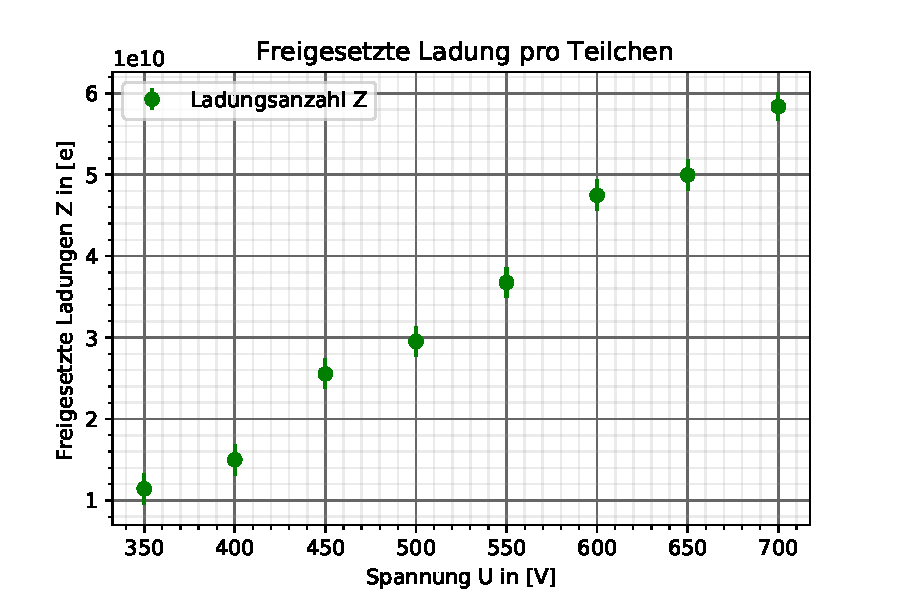
\includegraphics{ladungproteilchen.pdf}
  \caption{Pro einfallendem Teilchen ausgelöste Ladung}
  \label{fig:ladungProTeilchen}
\end{figure}
\begin{table}
\centering
    \caption{Ladungen pro einfallendem Teilchen}
    \sisetup{table-format=1.2}
    \begin{tabular}{S[table-format=3.2] S S S S  [table-format=3.2]}
      
      \toprule
      {$U$[V]} & {$N[e]$}\\
      \midrule
      350  &   {$11420877863  \pm 1906959500$}\\
      400  &   {$14987116964  \pm 1879377895$}\\
      450  &   {$25540082774  \pm 1841627474$}\\
      500  &   {$29513591578  \pm 1867714299$}\\
      550  &   {$36772445516  \pm 1874382573$}\\
      600  &   {$47482469587  \pm 1885491961$}\\
      650  &   {$49965388277  \pm 1849942326$}\\
      700  &   {$58377332056  \pm 1710174398$}\\
\bottomrule
    
    \end{tabular}
  \end{table}